
%% Title Page 
\title{\Huge Testing Spec\\ 
	 Project: \\ 
	Cafeteria Management System: Reslove}
\author{
         \underline{T-RISE}\\
          Rendani Dau (13381467) \\
	Elana Kuun (12029522) \\
	Semaka Malapane (13081129) \\
	Antonia Michael (13014171) \\
	Isabel Nel (13070305)}

\date{\today}

\documentclass[12pt]{article}

\begin{document}
\maketitle
\break

%% Make table of contents
\tableofcontents
\break

%%now begin document

%%---------------------------------  INTRODUCTION -------------------------------------------
\section{Introduction}
This document contains the functional requirements specification, architecture requirements and testing for the Resolve Cafeteria Management System that will be created for Software Engineering (COS 301) at the University of Pretoria 2015, by the group T-RISE. In this document we will thoroughly discuss and layout the project's testing to provide a clear view of the system as a whole. An agile approach is being followed, hence the main use cases that this document will be focussing on are placing orders and managing a user profile.  

%% ------------------------------ VISION ------------------------------------------------------
\section{Vision}
The vision of this project is to implement a flexible, pluggable, fully functional software application that will be maintainable, with detailed supporting documentation and an instruction manual for the Cafeteria Management System. This system will assist in managing the cafeteria's inventory/stock, executing orders from the cafeteria, generating bills and sending these to the appropriate parties and facilitating payments for access cards (or the use of unique access card numbers). 

%%---------------------------------- BACKGROUND -----------------------------------------
\section{Background}
As specified in the project proposal document from Resolve - the cafeteria is currently cash only and does not accept bank cards or electronic payments. This makes it inconvenient for employees as they have to carry around cash if they want to purchase anything from the cafeteria. Hence, this is equivalent to purchasing from an external food outlet where they can also pay with their preferred method of payment. The employees have to hence use up fuel and time and lastly this does not bring in the maximum amount of income to the cafeteria, hindering its growth and improvement.\\

Resolve is therefore looking for a means to accept payments from employees for the canteen using their employee access cards or access card numbers, with an amount being deducted from their salary at the end of the month.\\

Resolve proposed the Cafeteria Management System to assist with this problem.
After our first meeting with the client, they brought to our attention that at times the cafeteria does not even have enough stock to provide some of the menu items, thus the managing of inventory or stock will also be part of the system. The system will also predict what inventory/stock needs to be bought for the next week in order to avoid such a problem. At the end of each month, the bill for the month will be sent to either payroll or to the employee. This option is configurable from the user's profile. The employee can also set a spending limit for each month for control purposes. The system will have its own maximum, such that users cannot set a limit that exeeds this. 


%%-------------TESTING--------------------------------------
\subsection{Testing}

Testing for the two main use cases discussed in this document has been done using Mocha for unit testing. We have tested the various functions identified for the two different use cases. For placing an order, the functions that are to be created are checkProductAvailability, checkLimits, isLoggedIn and generateBill. 

Once the user has selected items to be purchased, the system needs to check that the user has logged in, so that using the employeeId the system will know which user's profile needs to be edited. The system has to then check whether the products are in stock and whether the total price of the items selected stays within the user's set limit. The bill is then generated, stating the items purchased and the cost.

These functions will return strings indicating whether the desired operation associated with them was successfully carried out or not. Mock Json objects consisting of the different parameters required for each function have been passed to the function in the tests. If the functions in the placeOrder.js file pass all these tests, the file will be able to be integrated into the rest of the system. 
\\
Due to the fact that an agile approach is being used, these unit tests might need to be edited if the functional requirements are edited along the way. Screenshots of some of the unit tests that have been created are displayed below. The entire unit test file can be found in the github repository in the unit test folder.  
\\
The second use case is manage profile, and the functions that have thus far been identified for this use case are editProfile, changePassword, changeEmail, setLimit, editRecipients, displayBill, viewHistory and generateFavourites. 
\\
The system must hence allow the logged in user to change their various settings, as well as allow the user to view the day's bill as well as the account history.
\\
A sample of the code from the unit testing file is displayed below.
%\begin{figure}[h!]
%\centering
%	 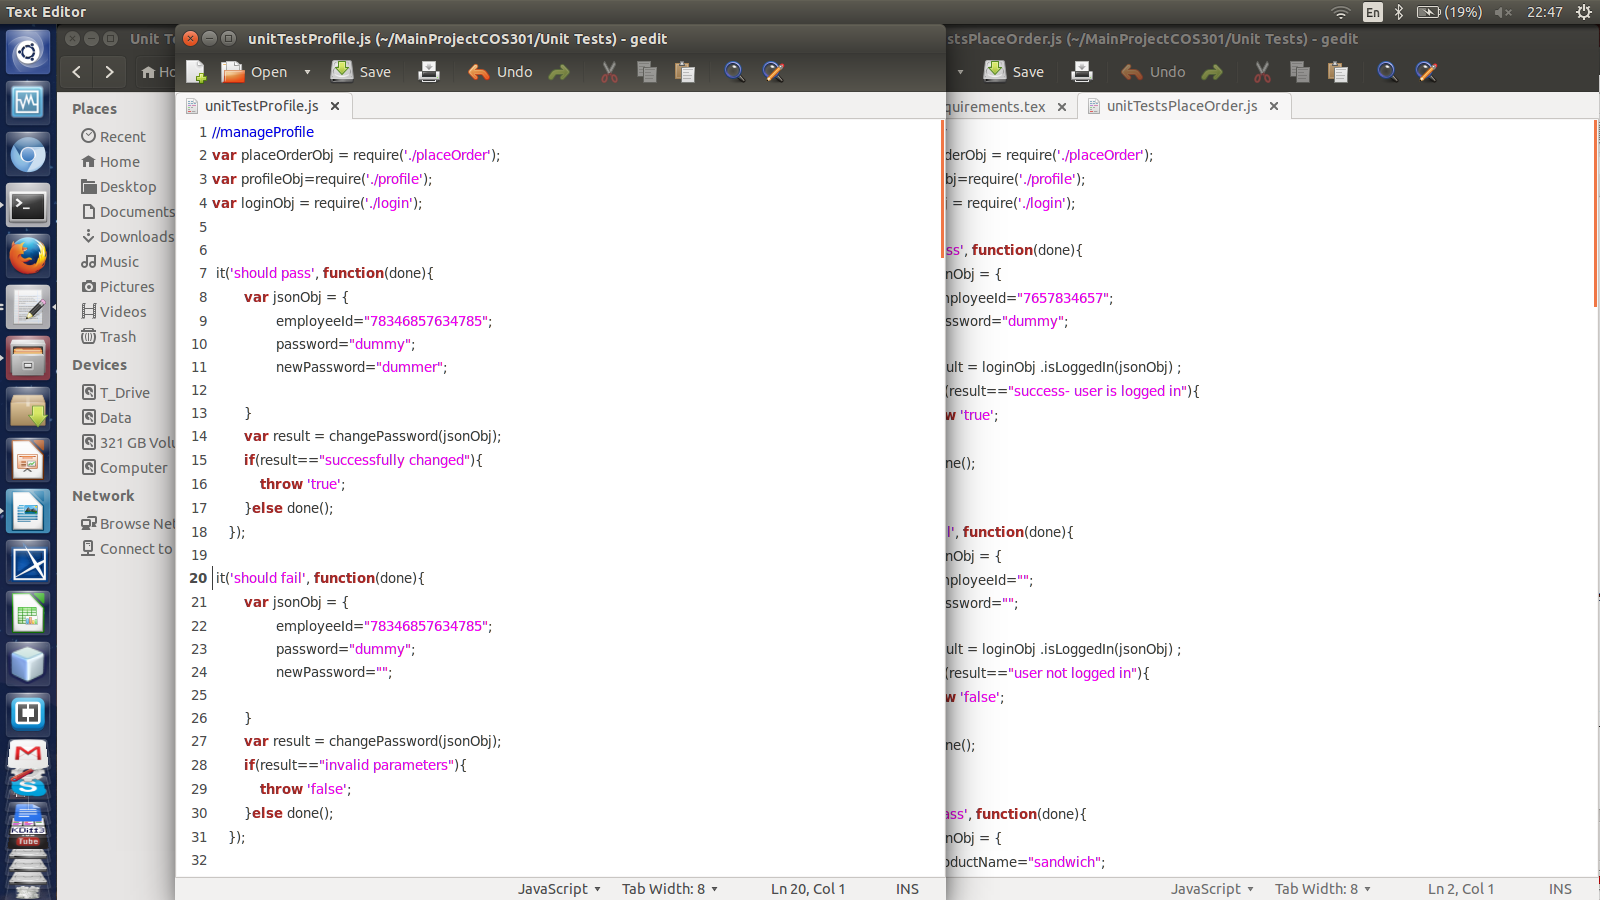
\includegraphics[width=1\textwidth]{./Unit Tests/unitTestScreenShots/profilePic.jpg}
%\end{figure}
